Although calculations above in section \ref{methods} show the Von Neumann entanglement entropy, the Renyi entanglement entropy is also a useful measure of entanglement. The Renyi entanglement entropy is defined as 
\begin{equation}
S_{\alpha} = \frac{1}{1-\alpha} \ln{\left( \text{Tr} \left( \rho_A^{\alpha} \right) \right)},
\end{equation}
where $\rho_A$ is the reduced density matrix of the subsystem $A$ and $\alpha$ is a parameter that can be varied. The Renyi entanglement entropy is a generalization of the Von Neumann entanglement entropy, which is the case when $\alpha \rightarrow 1$ [REF HERE (Wang, 2016)]. \cref*{fig:ed_renyi} is a graph of the $2_{nd}$ Renyi entanglement entropy (i.e., the case when $\alpha = 2$) versus the ratio of the interaction term ($U$) to the hopping term ($J$).

\begin{figure}[H]
\centering
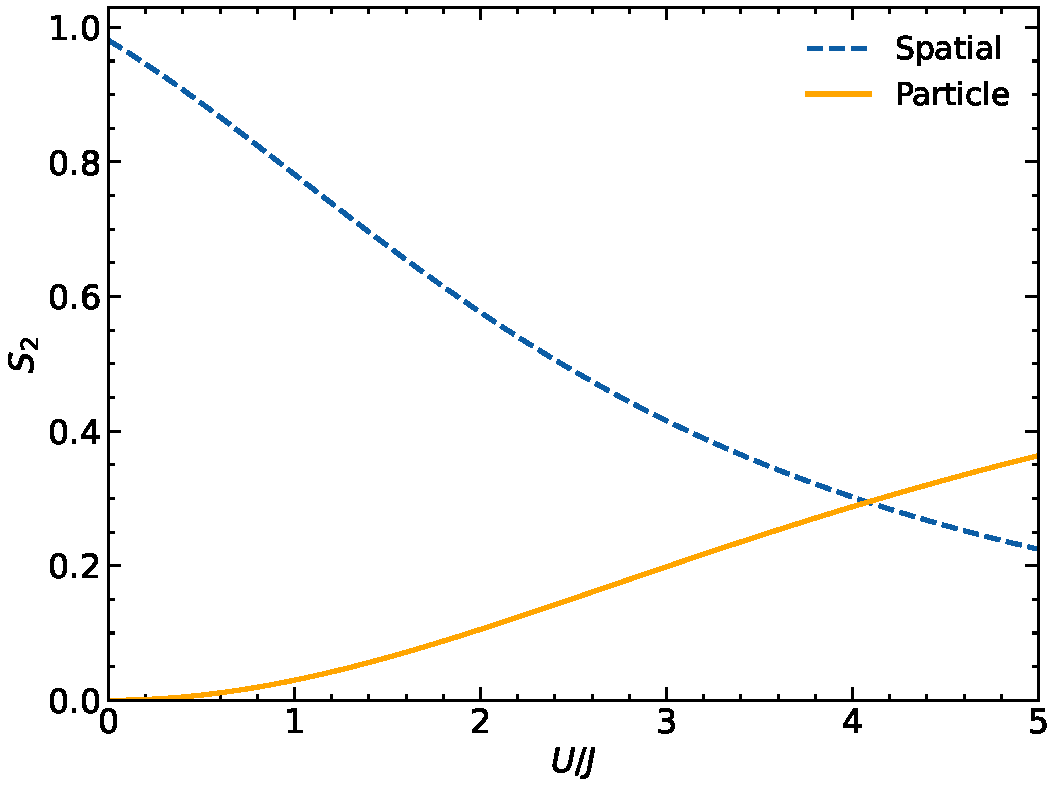
\includegraphics[scale=0.5]{../figures/ed_renyi.pdf}
\caption{The figure above is a graph of the Renyi entanglement entropy for both spatial and particle bipartitions versus the ratio of the interaction term to the hopping term.}
\label{fig:ed_renyi}
\end{figure}

\subsection{PIGSFLI Algorithm} \label{PIGSFLI}

A Monte Carlo simulation is a stochastic (random) method of integration, which allows for accurate estimations of desired values. Monte Carlo is necessary for situations where exact calculations are too computationally expensive, such as in the exact diagonalization of the reduced density matrix for high particle/site number Bose Hubbard systems. For example, the size of the Hilbert space is calculated by \cref{eq:36} and shown by \cref{fig:hilbert_space_size}:

\begin{equation}
D = \frac{\left(N+L-1\right)!}{\left(N\right)!\left(L-1\right)!}.
\label{eq:36}
\end{equation}

In this example, the Hilbert space size is calculated for a system with $N$ particles and $L$ sites. The Hilbert space size is the number of possible states that the system can be in. For example, a system with $N=2$ particles and $L=2$ sites has a Hilbert space size of $3$. This means that there are $3$ possible states that the system can be in. The largest system size shown by \cref{fig:hilbert_space_size} is $20$ particles and $20$ sites, which has a Hilbert space size of $6.8 \times 10^{10}$ or about 68 billion possible states. For this reason, exact diagonalization is not feasible for large system sizes and Monte Carlo methods are necessary with classical computation.

\begin{figure}[H]
\centering
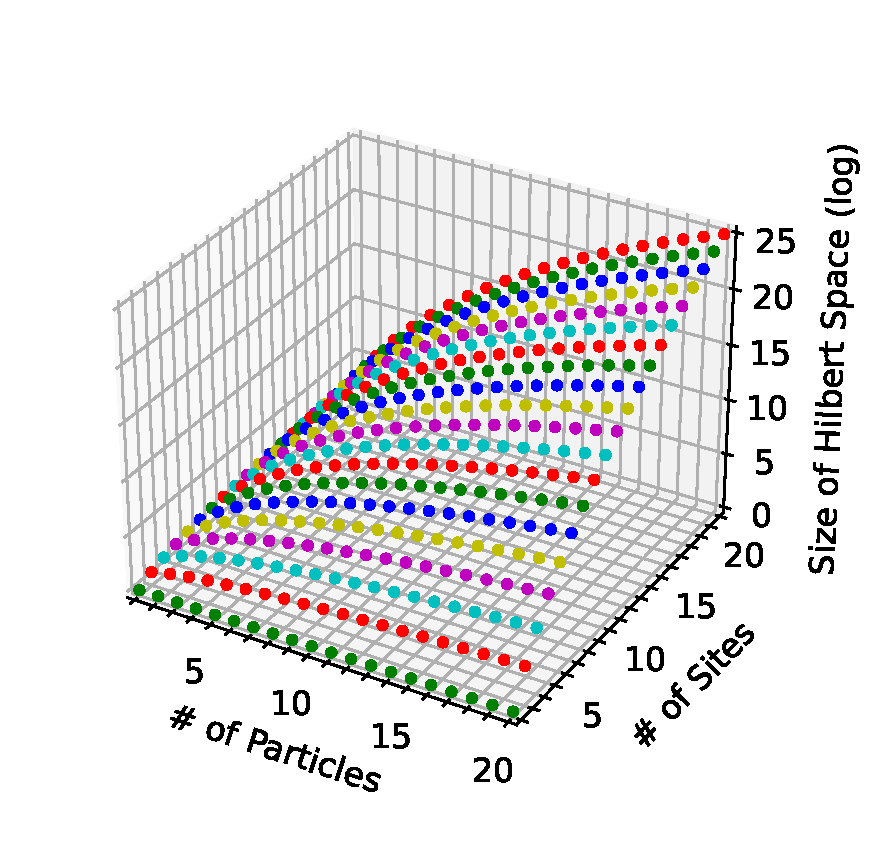
\includegraphics[scale=0.5]{../figures/hilbert_space_size.pdf}
\caption{The figure above shows the size of the Hilbert space as a function of number of sites and particles. This 3-dimensional plot for the number of combinations in the Hilbert space goes up to $20$ sites and $20$ particles.}
\label{fig:hilbert_space_size}
\end{figure}

\cref*{fig:total_energy} shows the total (both kinetic and potential) ground state energy of the 2 particle, 2 site system versus the ratio of the interaction term ($U$) to the hopping term ($J$). More specifically, this plot contains both data points generated by the PIGSFLI algorithm and the curve we would expect theoretically from adding the expectation values of both the kinetic and potential energies. The expecation values of the kinetic and potential energies are as follows: 
\begin{align*}
    K.E. &= \langle \psi | \hat{H}_K | \psi \rangle \\
    P.E. &= \langle \psi | \hat{H}_P | \psi \rangle
\end{align*}
\begin{figure}[H]
\centering
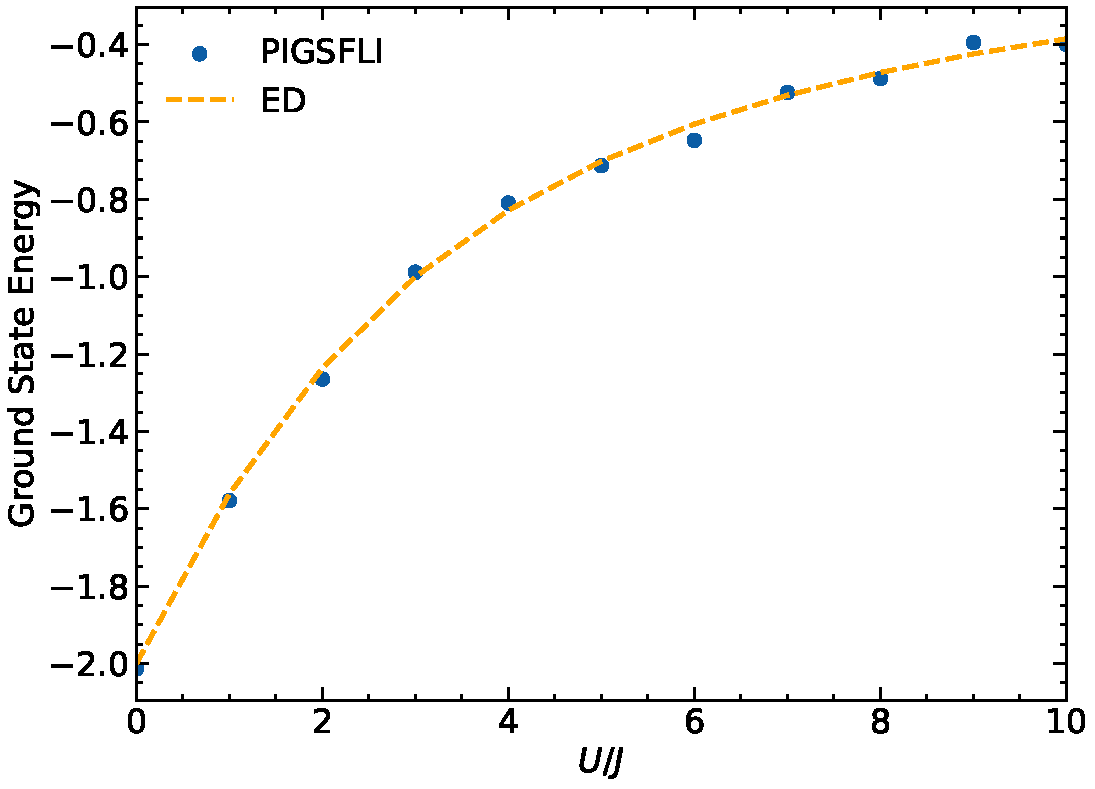
\includegraphics[scale=0.5]{../figures/total_energy.pdf}
\caption{A plot of the ground state energy versus the ratio between U, the potential term, and J, the hopping term for both exact diagonalization and PIGSFLI algorithm. From this plot, the PIGSFLI reults match very well to our ED calculation.}
\label{fig:total_energy}
\end{figure}

A good way to ensure the PIGSFLI algorithm appears correct from a general physics sense, it is important to look at the occupancy graphs for each site: occupancy is essentially the probability of that site being occupied by a particle. These plots are shown in \cref{fig:sep_occ_hist_U_0.0001,fig:spatial_avg_occ_U_0.0001,fig:sep_occ_hist_U_10.0000,fig:spatial_avg_occ_U_10.0000} below. 

The first two plots show the case where the interaction term is small. Since the interaction term is repulsive, the particles should exist on the sites with equal probability.

\begin{figure}[H]
\centering
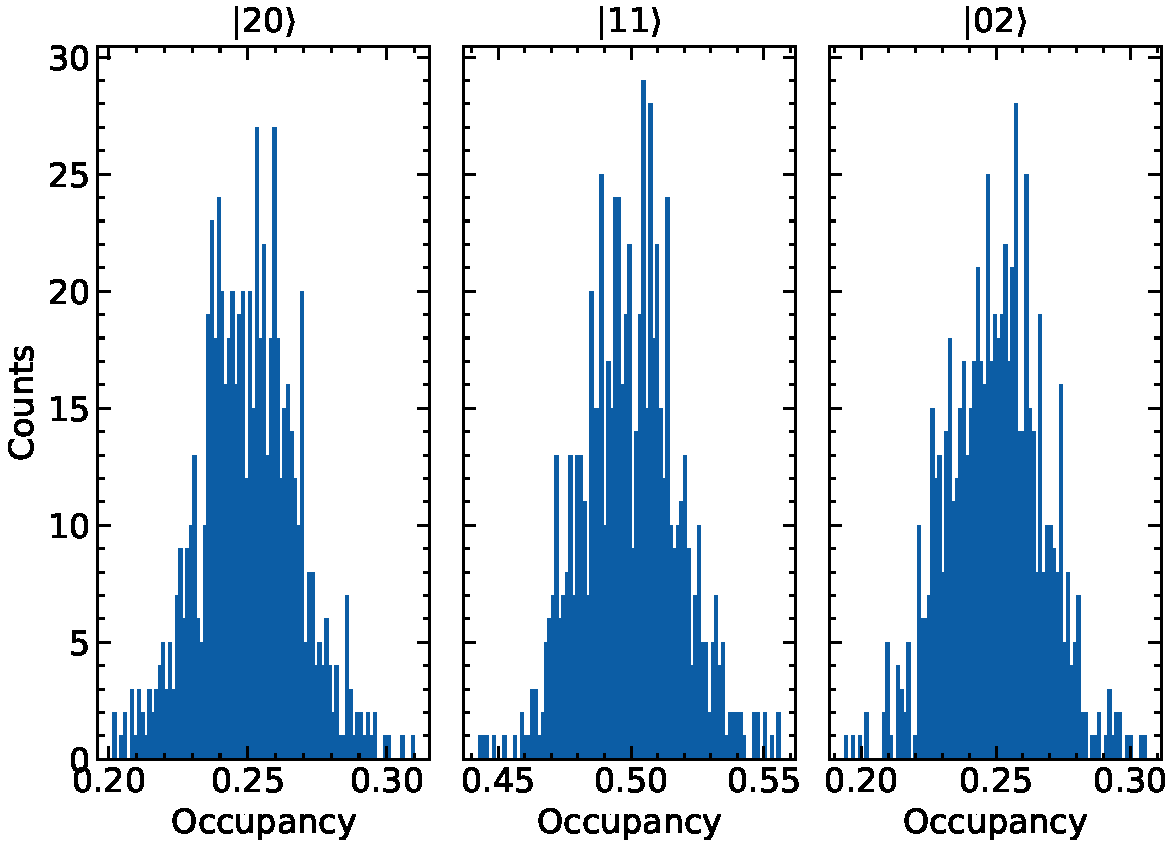
\includegraphics[scale=0.5]{../figures/sep_occ_hist_U_0.0001.pdf}
\caption{The figure above shows the histogram of the occupation number for the particle bipartition as a function of the ratio of the interaction term to the hopping term. This graph specifically shows the case where the interaction term is a tenth of the hopping term.}
\label{fig:sep_occ_hist_U_0.0001}
\end{figure}

\begin{figure}[H]
\centering
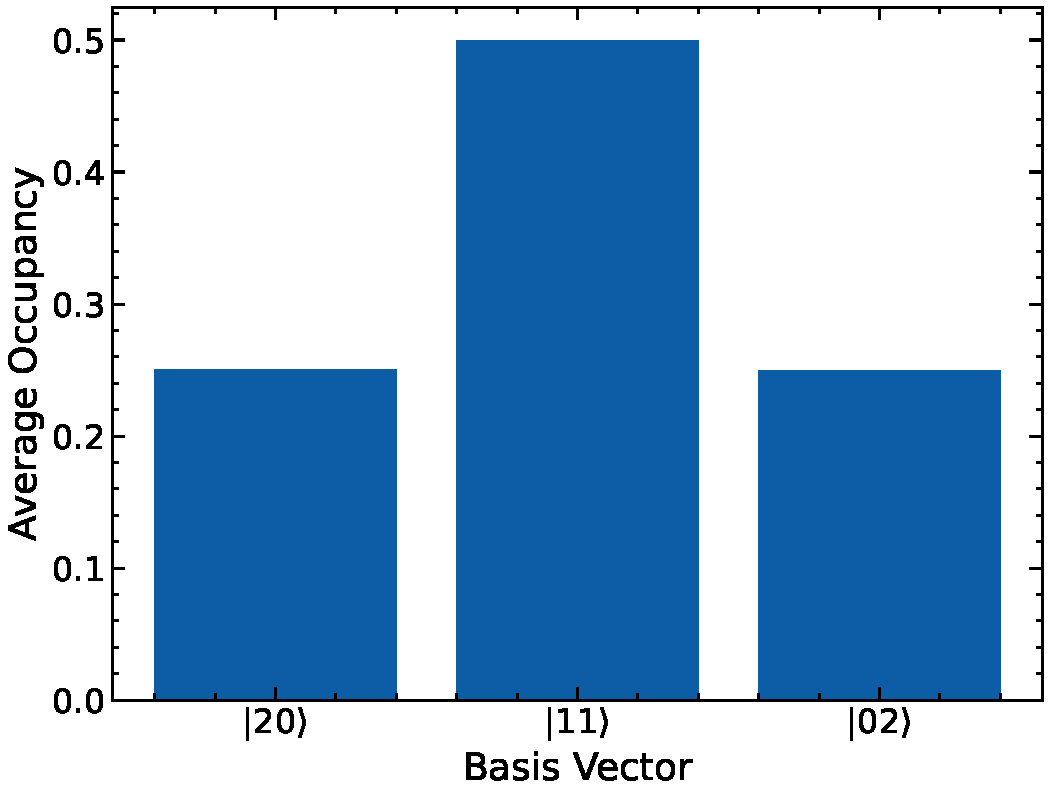
\includegraphics[scale=0.5]{../figures/spatial_avg_occ_U_0.0001.pdf}
\caption{The figure above shows the average occupation number for the spatial bipartition as a function of the ratio of the interaction term to the hopping term. This graph specifically shows the case where the interaction term is a tenth of the hopping term.}
\label{fig:spatial_avg_occ_U_0.0001}
\end{figure}

The second two plots show the case where the interaction is much larger. Since the interaction term is repulsive, the particles should converge on the $|11\rangle$ state: the state where they exist the farthest distance from each other.

\begin{figure}[H]
\centering
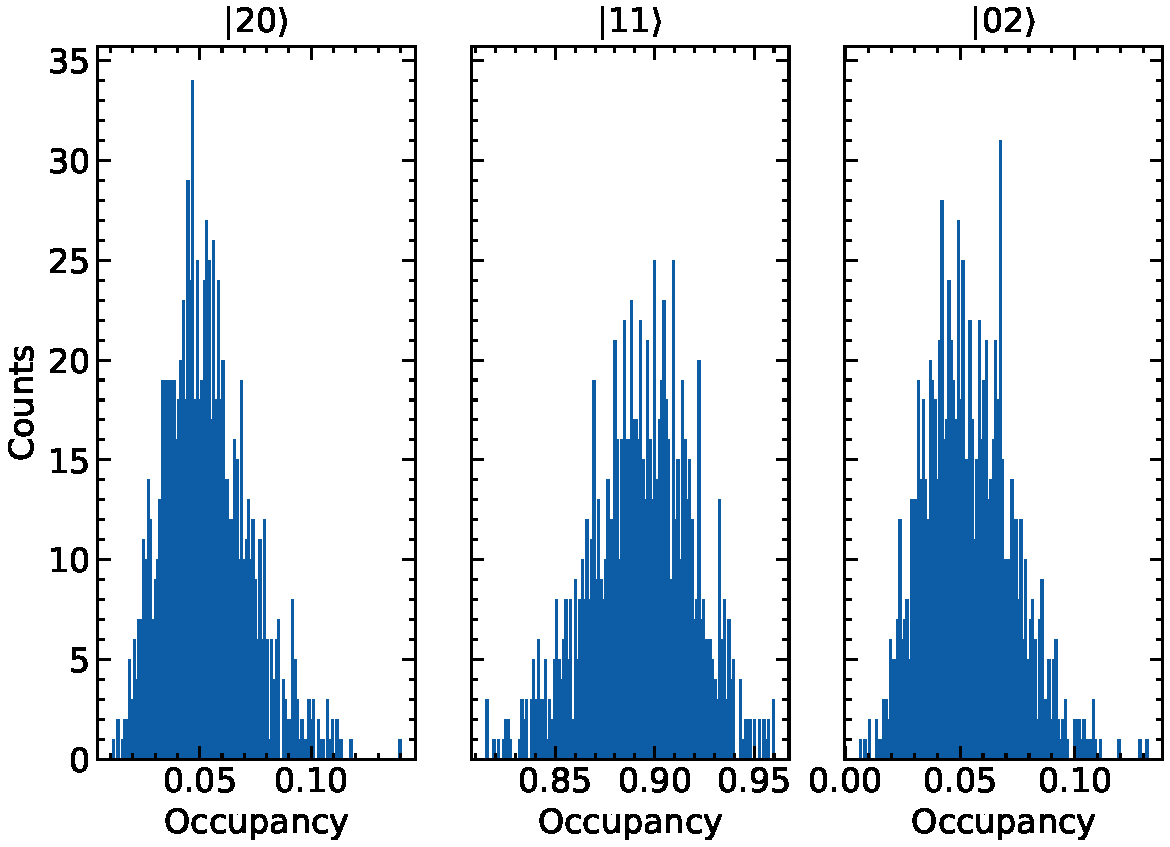
\includegraphics[scale=0.5]{../figures/sep_occ_hist_U_10.0000.pdf}
\caption{The figure above shows the histogram of the occupation number for the spatial bipartition as a function of the ratio of the interaction term to the hopping term. This graph specifically shows the case where the interaction term is $10$ times the hopping term.}
\label{fig:sep_occ_hist_U_10.0000}
\end{figure}

\begin{figure}[H]
\centering
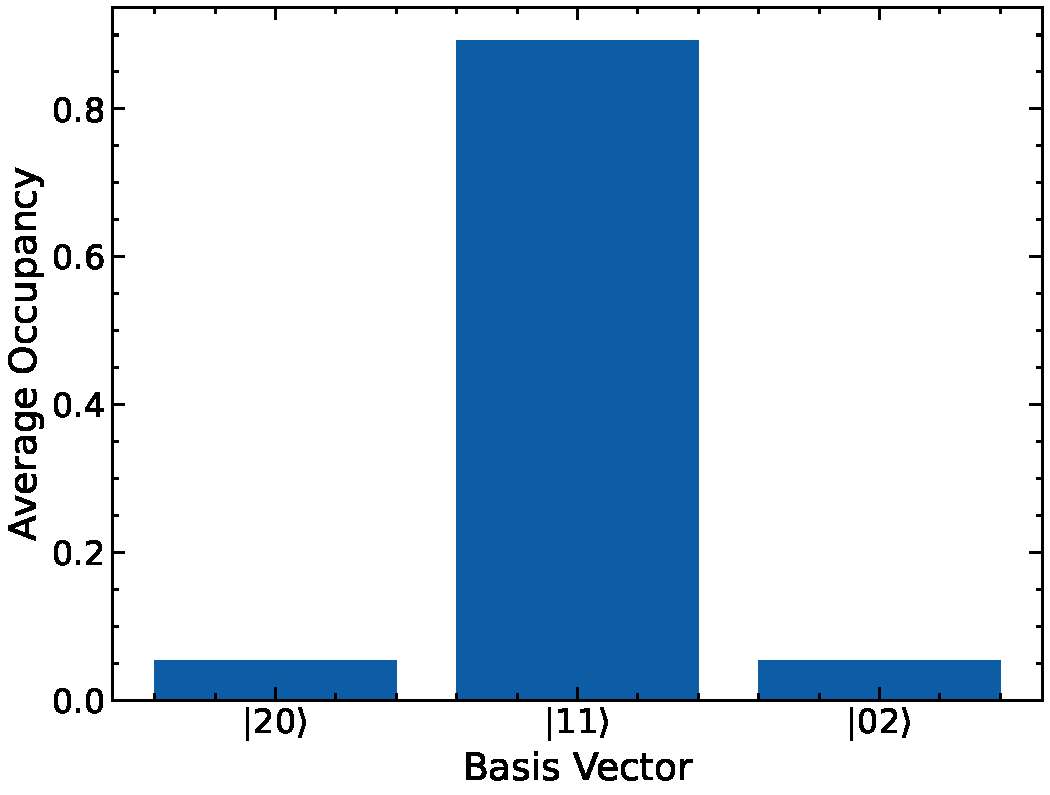
\includegraphics[scale=0.5]{../figures/spatial_avg_occ_U_10.0000.pdf}
\caption{The figure above shows the average occupation number for the spatial bipartition as a function of the ratio of the interaction term to the hopping term. This graph specifically shows the case where the interaction term is $10$ times the hopping term.}
\label{fig:spatial_avg_occ_U_10.0000}    
\end{figure}

\subsubsection{Comparison of PIGSFLI to Exact Diagonalization} \label{results}

\cref*{fig:renyi_spatial} is a plot of the second Renyi entanglement entropy versus the ratio of the interaction term ($J$) to the hopping term ($U$). More specifically, this plot contains both data points generated by the PIGSFLI algorithm and the curve we would expect theoretically from \cref{eq:36}.

\begin{figure}[H]
\centering
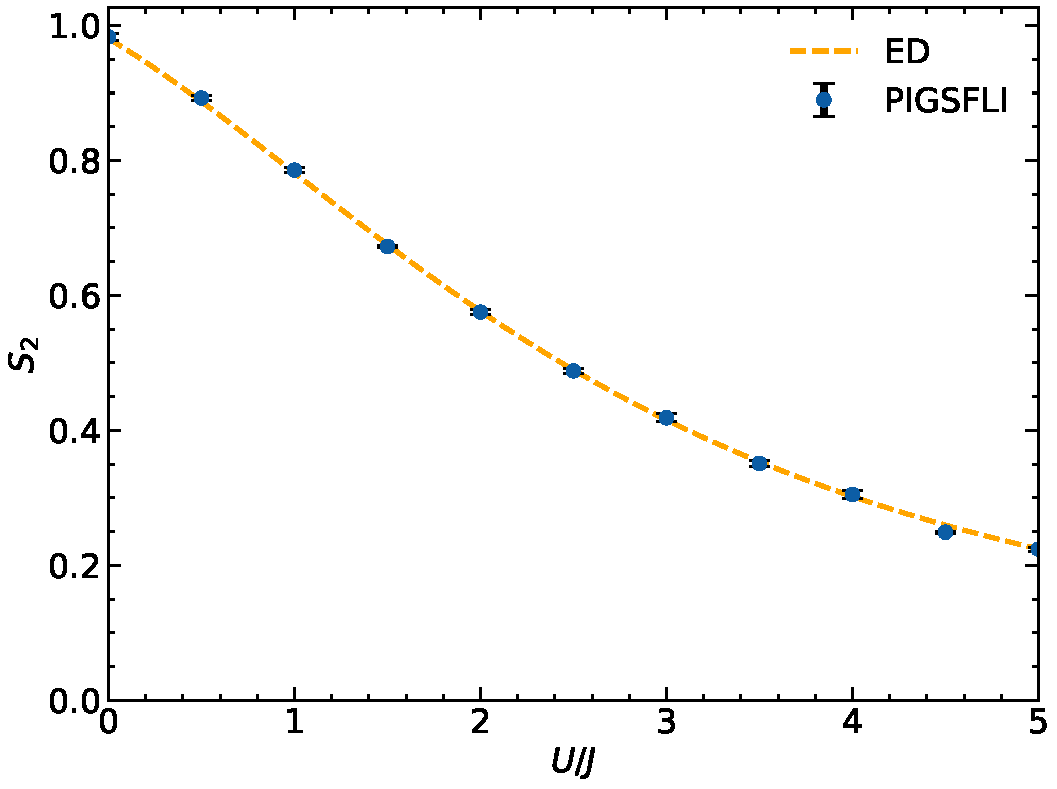
\includegraphics[scale=0.5]{../figures/renyi_spatial.pdf}
\caption{The second Rényi spatial entanglement entropy as a function of U/J for both exact diagonalization (ED) and PIGSFLI. This plot shows excellent agreement between the PIGSFLI estimation and that of our ED calculation, showing that PIGSFLI is a viable option for computation on much larger system sizes.}
\label{fig:renyi_spatial}
\end{figure}

\subsection{Introduction to Machine Learning for Scientists}
While working with the DelMaestro group and attending lectures held during the QAO REU at the University of Tennessee Koxville, I was exposed to machine learning as a tool for physicists and other scientists alike. 

\subsubsection{Applications of DNN to Physics}
\begin{description}
\item [Application:] Learning the Energy Potential
\item [Description:] Train network on small system sizes (which we know the exact solution for), then extrapolate for application of larger system sizes.

\item [Application:] Phase Discrimination
\item [Description:] Supervised and un-supervised machine learning used to classify phases of matter.

\item[Application:] Variational Ansatz 
\item[Description:] Method of guessing the wave function to solve the Schrodinger equation for a given potential quickly.

\item [Application:] Solving the Schrodinger Equation
\item[Description:] Train a neural network to solve the Schrodinger equation for a given potential.

\item [Application:] Speeding up Monte Carlo
\item [Description:] Monte Carlo update algorithms are highly dependent on the model. Therefore, a neural network can be trained to predict the next state of the system, which can speed up the Monte Carlo simulation.
\end{description}

\subsubsection{Basic Neural Networks}
\begin{figure}[H]
\centering
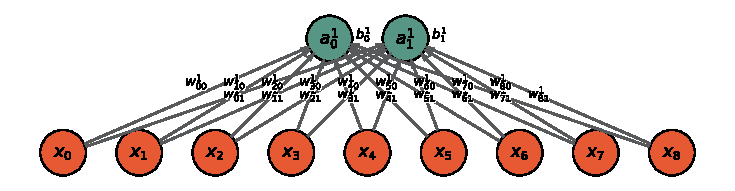
\includegraphics{../figures/neural_network.pdf}
\caption{The figure above is an example of a simple feed-forward neural network, taking in nine inputs and returning two outputs.}
\end{figure}

\noindent \textbf{Neural Network:} non-linear function of many variables that depends on a large number of parameters \\
\textbf{Deep Neural Network:} a neural network with one or more hidden layers (i.e., not an input or output layer)

\begin{figure}[H]
\centering
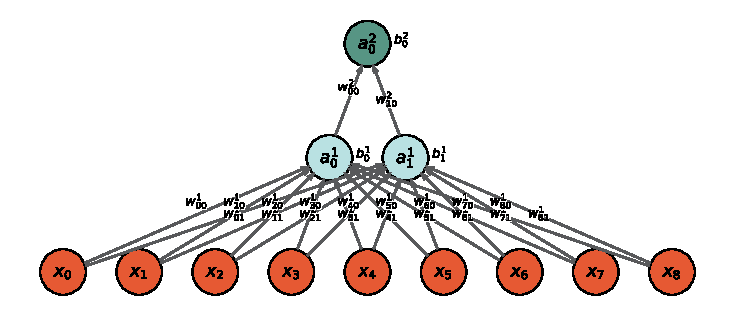
\includegraphics{../figures/DNN.pdf}
\caption{The figure above is an example of a simple feed-forward deep neural network, taking in nine inputs and returning one output with one hidden layer between the input and output layers.}
\end{figure}
			
\subsubsection{Visualizing Feed Forward}
Some examples to visualize complexity generated from simple feed forward neural network with 2 input parameters and 2 hidden layers with 200 nodes each are shown below:

\begin{figure}[H]
\centering
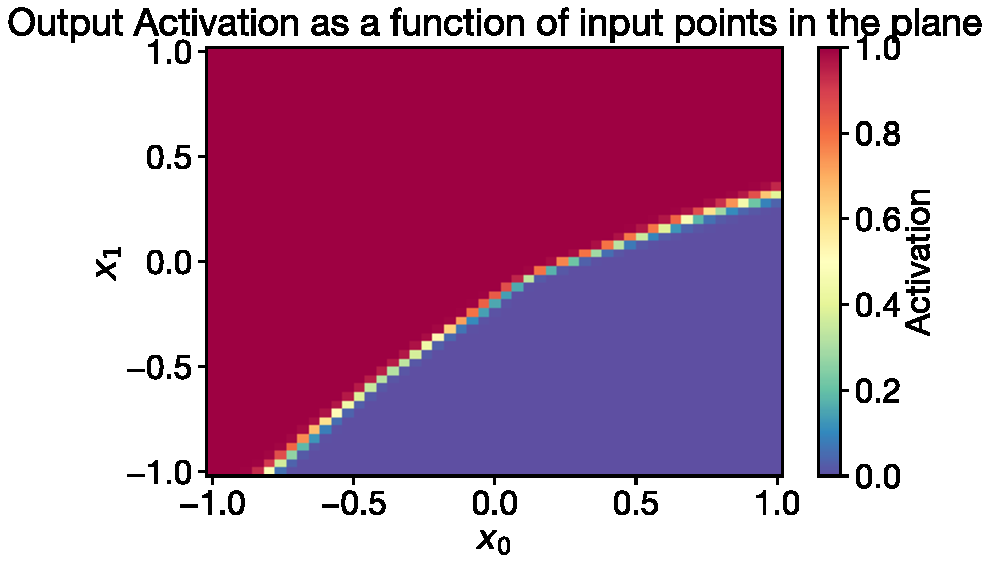
\includegraphics[scale=0.65]{../figures/activation_heat_map.pdf}
\caption{The figure above is the activation output as a function of the two input parameters $x_0$ and $x_1$, which were randomly generated. The activation is calculated through use of the sigmoid function. Specifically, this is a heat map where the color is associated with the activation level.}
\end{figure}

\begin{figure}[H]
\centering
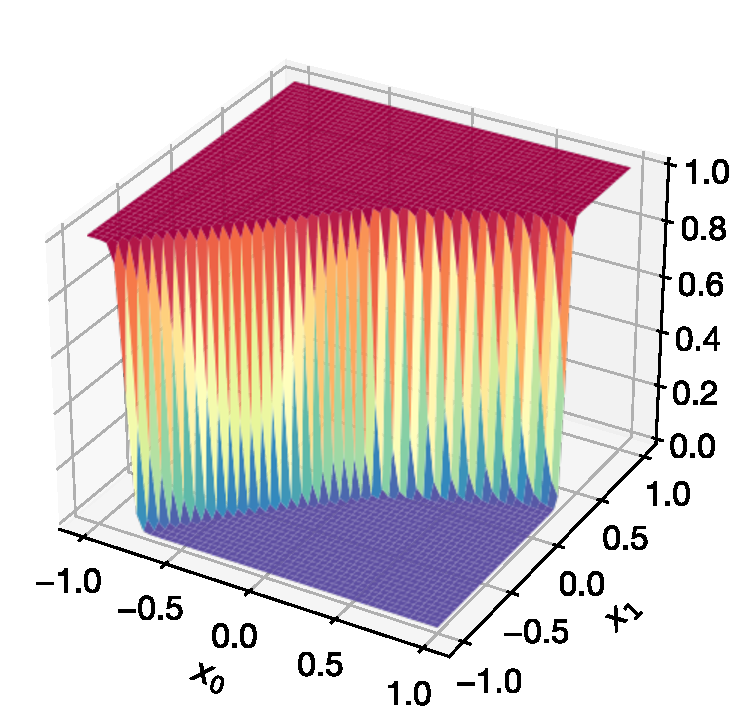
\includegraphics[scale=0.65]{../figures/activation_3d.pdf}
\caption{The figure above is the activation output as a function of the two parameters $x_0$ and $x_1$, which were randomly generated. The activation is calculated through use of the sigmoid function. Specifically, this is a heat map in 3-dimensional space where the activation is the on the vertical axis.}
\end{figure}

\subsubsection{Batch Processing}

Multiple batches of data can be processed at once, which can be more efficient than processing one set of data at a time. This is especially useful when running the neural network on a GPU, which can process multiple batches of data in parallel. The most common way of achieving batch processing is through linear algebra methods with Numpy, which is a Python library for numerical computing.

\subsubsection{Linear Regression}
\subsubsubsection{Linear Regression Example}
The radioactive decay of an unknown sample is described by the following equation:
\begin{equation}
N(t) = N(0) e^{-t/\tau},
\end{equation}
where $N(t)$ is the number of atoms at time $t$, $N(0)$ is the number of atoms at time $t=0$, $t$ is the time in seconds, and $\tau$ is the time constant of the decay. The above equation can be rearranged into a linear relationship of the form 
\begin{equation}
N(t) = \ln{\left( N(0) \right)} - \frac{1}{\tau}t.
\end{equation}
For our simple feed forward neural network, this is similar to the following form:
\begin{equation}
F = w_o + w_1t,
\end{equation}
were $F$ is the function we're trying to fit, $w_0$ and $w_1$ are the weights, which are (potentially non-linear) functions of the unknown parameters $N(0)$ and $\tau$, and $t$ is the time in seconds. Plotting the original data as well as the linear regression calculation, we find the following:
\begin{figure}[H]
\centering
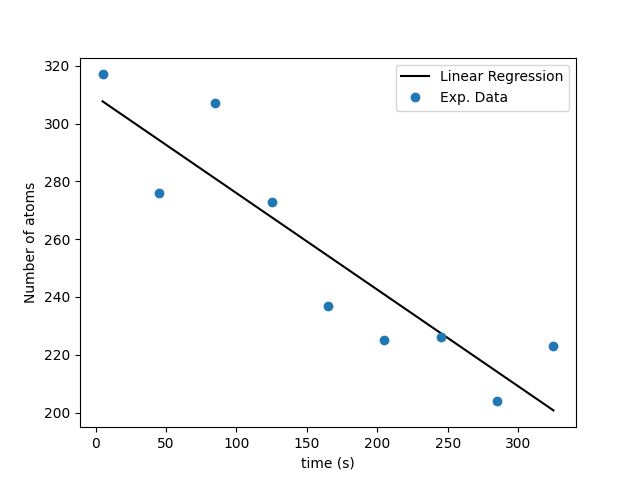
\includegraphics[scale=0.75]{../figures/decay_data.png}
\caption{This figure is a plot of the number of atoms versus time passed in seconds. The blue data points in the figure above represent the experimental data and the black line represents the linear fit to this data using a simple feed-forward neural network.}
\end{figure}